\documentclass[tikz,border=3mm,multi=tikzpicture]{standalone}
\usepackage{tikz}
\usetikzlibrary{arrows.meta}
\begin{document}
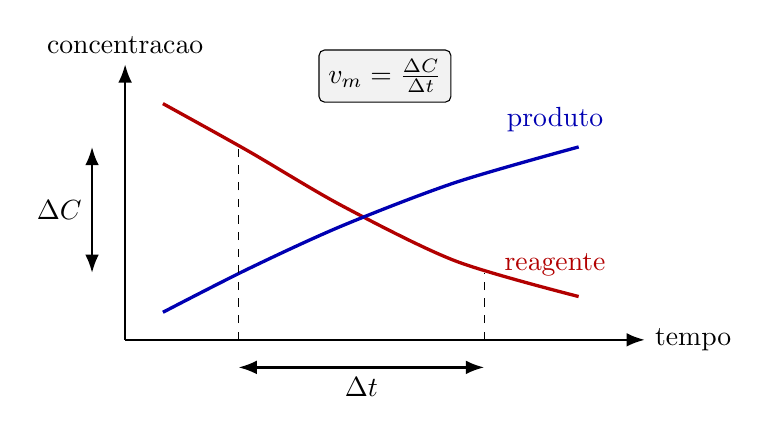
\begin{tikzpicture}[x=1.2cm,y=1cm,>=Latex]
  \draw[->,thick] (0,0) -- (5.5,0) node[right] {tempo};
  \draw[->,thick] (0,0) -- (0,3.5) node[above] {concentracao};
  \draw[very thick,red!70!black] plot[smooth] coordinates {(0.4,3.0) (1.3,2.4) (2.3,1.7) (3.5,1.0) (4.8,0.55)};
  \draw[very thick,blue!70!black] plot[smooth] coordinates {(0.4,0.35) (1.3,0.9) (2.3,1.45) (3.5,2.0) (4.8,2.45)};
  \node[red!70!black] at (4.55,0.95) {reagente};
  \node[blue!70!black] at (4.55,2.8) {produto};
  \draw[dashed] (1.2,0) -- (1.2,2.5);
  \draw[dashed] (3.8,0) -- (3.8,0.85);
  \draw[<->,thick] (1.2,-0.35) -- (3.8,-0.35) node[midway,below] {$\Delta t$};
  \draw[<->,thick] (-0.35,2.45) -- (-0.35,0.85) node[midway,left] {$\Delta C$};
  \node[draw,rounded corners=2pt,fill=gray!10,align=center] at (2.75,3.35) {$v_m=\frac{\Delta C}{\Delta t}$};
\end{tikzpicture}

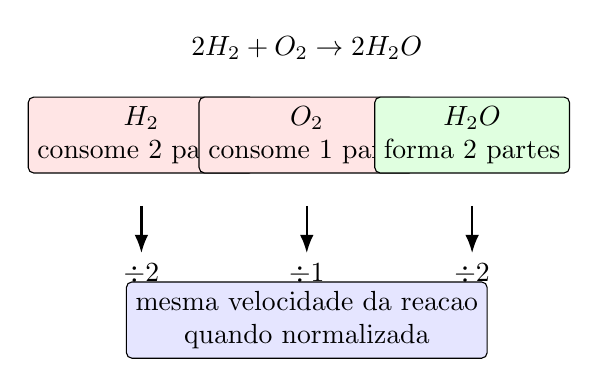
\begin{tikzpicture}[x=1cm,y=1cm,>=Latex]
  \draw[very thick] (0,0) -- (6.2,0);
  \node[align=center] at (3.1,1.45) {$2H_2 + O_2 \rightarrow 2H_2O$};
  \node[draw,rounded corners=2pt,fill=red!10,align=center] at (1.0,0.35) {$H_2$\\consome 2 partes};
  \node[draw,rounded corners=2pt,fill=red!10,align=center] at (3.1,0.35) {$O_2$\\consome 1 parte};
  \node[draw,rounded corners=2pt,fill=green!12,align=center] at (5.2,0.35) {$H_2O$\\forma 2 partes};
  \draw[->,thick] (1.0,-0.55) -- (1.0,-1.15) node[below] {$\div 2$};
  \draw[->,thick] (3.1,-0.55) -- (3.1,-1.15) node[below] {$\div 1$};
  \draw[->,thick] (5.2,-0.55) -- (5.2,-1.15) node[below] {$\div 2$};
  \node[draw,rounded corners=2pt,fill=blue!10,align=center] at (3.1,-2.0) {mesma velocidade da reacao\\quando normalizada};
\end{tikzpicture}
\end{document}
